\chapter{Instant Insanity Puzzle}

Rishnak was examining the headstones of some of the graves. He saw a headstone with a name Schossow \footnote{ Schossow got a ptent for proposing this puzzle in 1899\url{https://patents.google.com/patent/US646463A/en} }  in a grave. That brought him memories of the puzzle called the Great Tantalizer (also known as Instant Insanity).
Rishnak thought that was a great puzzle to tell Ajur as this puzzle have a nice graph theoretic solution.
\begin{figure}
\begin{center}
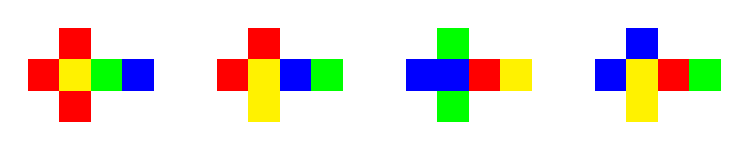
\begin{tikzpicture}
[scale=.8]
%First Cube
\fill [red] (0.0,0.0) rectangle (0.5,0.5);
\fill [yellow] (0.5,0.0) rectangle (1.0,0.5);
\fill [green] (1.0,0.0) rectangle (1.5,0.5);
\fill [blue] (1.5,0.0) rectangle (2.0,0.5);
\fill [red] (0.5,-0.5) rectangle (1.0,0.0);
\fill [red] (0.5,0.5) rectangle (1.0,1.0);
%Second Cube
\fill [red] (3.0,0.0) rectangle (3.5,0.5);
\fill [yellow] (3.5,0.0) rectangle (4.0,0.5);
\fill [blue] (4.0,0.0) rectangle (4.5,0.5);
\fill [green] (4.5,0.0) rectangle (5.0,0.5);
\fill [yellow] (3.5,-0.5) rectangle (4.0,0.0);
\fill [red] (3.5,0.5) rectangle (4.0,1.0);
%Third  Cube
\fill [blue] (6.0,0.0) rectangle (6.5,0.5);
\fill [blue] (6.5,0.0) rectangle (7.0,0.5);
\fill [red] (7.0,0.0) rectangle (7.5,0.5);
\fill [yellow] (7.5,0.0) rectangle (8.0,0.5);
\fill [green] (6.5,-0.5) rectangle (7.0,0.0);
\fill [green] (6.5,0.5) rectangle (7.0,1.0);
%Fourth Cube
\fill [blue] (9.0,0.0) rectangle (9.5,0.5);
\fill [yellow] (9.5,0.0) rectangle (10.0,0.5);
\fill [red] (10.0,0.0) rectangle (10.5,0.5);
\fill [green] (10.5,0.0) rectangle (11.0,0.5);
\fill [yellow] (9.5,-0.5) rectangle (10.0,0.0);
\fill [blue] (9.5,0.5) rectangle (10.0,1.0);
\end{tikzpicture}
\caption{ Four Cubes}\label{21p1}
\end{center}
\end{figure}